% Options for packages loaded elsewhere
\PassOptionsToPackage{unicode}{hyperref}
\PassOptionsToPackage{hyphens}{url}
%
\documentclass[
]{article}
\usepackage{lmodern}
\usepackage{amssymb,amsmath}
\usepackage{ifxetex,ifluatex}
\ifnum 0\ifxetex 1\fi\ifluatex 1\fi=0 % if pdftex
  \usepackage[T1]{fontenc}
  \usepackage[utf8]{inputenc}
  \usepackage{textcomp} % provide euro and other symbols
\else % if luatex or xetex
  \usepackage{unicode-math}
  \defaultfontfeatures{Scale=MatchLowercase}
  \defaultfontfeatures[\rmfamily]{Ligatures=TeX,Scale=1}
\fi
% Use upquote if available, for straight quotes in verbatim environments
\IfFileExists{upquote.sty}{\usepackage{upquote}}{}
\IfFileExists{microtype.sty}{% use microtype if available
  \usepackage[]{microtype}
  \UseMicrotypeSet[protrusion]{basicmath} % disable protrusion for tt fonts
}{}
\makeatletter
\@ifundefined{KOMAClassName}{% if non-KOMA class
  \IfFileExists{parskip.sty}{%
    \usepackage{parskip}
  }{% else
    \setlength{\parindent}{0pt}
    \setlength{\parskip}{6pt plus 2pt minus 1pt}}
}{% if KOMA class
  \KOMAoptions{parskip=half}}
\makeatother
\usepackage{xcolor}
\IfFileExists{xurl.sty}{\usepackage{xurl}}{} % add URL line breaks if available
\IfFileExists{bookmark.sty}{\usepackage{bookmark}}{\usepackage{hyperref}}
\hypersetup{
  pdftitle={Urdu Language Sentiment Classifier},
  pdfauthor={Dan S. Reznik},
  hidelinks,
  pdfcreator={LaTeX via pandoc}}
\urlstyle{same} % disable monospaced font for URLs
\usepackage[margin=1in]{geometry}
\usepackage{color}
\usepackage{fancyvrb}
\newcommand{\VerbBar}{|}
\newcommand{\VERB}{\Verb[commandchars=\\\{\}]}
\DefineVerbatimEnvironment{Highlighting}{Verbatim}{commandchars=\\\{\}}
% Add ',fontsize=\small' for more characters per line
\usepackage{framed}
\definecolor{shadecolor}{RGB}{248,248,248}
\newenvironment{Shaded}{\begin{snugshade}}{\end{snugshade}}
\newcommand{\AlertTok}[1]{\textcolor[rgb]{0.94,0.16,0.16}{#1}}
\newcommand{\AnnotationTok}[1]{\textcolor[rgb]{0.56,0.35,0.01}{\textbf{\textit{#1}}}}
\newcommand{\AttributeTok}[1]{\textcolor[rgb]{0.77,0.63,0.00}{#1}}
\newcommand{\BaseNTok}[1]{\textcolor[rgb]{0.00,0.00,0.81}{#1}}
\newcommand{\BuiltInTok}[1]{#1}
\newcommand{\CharTok}[1]{\textcolor[rgb]{0.31,0.60,0.02}{#1}}
\newcommand{\CommentTok}[1]{\textcolor[rgb]{0.56,0.35,0.01}{\textit{#1}}}
\newcommand{\CommentVarTok}[1]{\textcolor[rgb]{0.56,0.35,0.01}{\textbf{\textit{#1}}}}
\newcommand{\ConstantTok}[1]{\textcolor[rgb]{0.00,0.00,0.00}{#1}}
\newcommand{\ControlFlowTok}[1]{\textcolor[rgb]{0.13,0.29,0.53}{\textbf{#1}}}
\newcommand{\DataTypeTok}[1]{\textcolor[rgb]{0.13,0.29,0.53}{#1}}
\newcommand{\DecValTok}[1]{\textcolor[rgb]{0.00,0.00,0.81}{#1}}
\newcommand{\DocumentationTok}[1]{\textcolor[rgb]{0.56,0.35,0.01}{\textbf{\textit{#1}}}}
\newcommand{\ErrorTok}[1]{\textcolor[rgb]{0.64,0.00,0.00}{\textbf{#1}}}
\newcommand{\ExtensionTok}[1]{#1}
\newcommand{\FloatTok}[1]{\textcolor[rgb]{0.00,0.00,0.81}{#1}}
\newcommand{\FunctionTok}[1]{\textcolor[rgb]{0.00,0.00,0.00}{#1}}
\newcommand{\ImportTok}[1]{#1}
\newcommand{\InformationTok}[1]{\textcolor[rgb]{0.56,0.35,0.01}{\textbf{\textit{#1}}}}
\newcommand{\KeywordTok}[1]{\textcolor[rgb]{0.13,0.29,0.53}{\textbf{#1}}}
\newcommand{\NormalTok}[1]{#1}
\newcommand{\OperatorTok}[1]{\textcolor[rgb]{0.81,0.36,0.00}{\textbf{#1}}}
\newcommand{\OtherTok}[1]{\textcolor[rgb]{0.56,0.35,0.01}{#1}}
\newcommand{\PreprocessorTok}[1]{\textcolor[rgb]{0.56,0.35,0.01}{\textit{#1}}}
\newcommand{\RegionMarkerTok}[1]{#1}
\newcommand{\SpecialCharTok}[1]{\textcolor[rgb]{0.00,0.00,0.00}{#1}}
\newcommand{\SpecialStringTok}[1]{\textcolor[rgb]{0.31,0.60,0.02}{#1}}
\newcommand{\StringTok}[1]{\textcolor[rgb]{0.31,0.60,0.02}{#1}}
\newcommand{\VariableTok}[1]{\textcolor[rgb]{0.00,0.00,0.00}{#1}}
\newcommand{\VerbatimStringTok}[1]{\textcolor[rgb]{0.31,0.60,0.02}{#1}}
\newcommand{\WarningTok}[1]{\textcolor[rgb]{0.56,0.35,0.01}{\textbf{\textit{#1}}}}
\usepackage{graphicx}
\makeatletter
\def\maxwidth{\ifdim\Gin@nat@width>\linewidth\linewidth\else\Gin@nat@width\fi}
\def\maxheight{\ifdim\Gin@nat@height>\textheight\textheight\else\Gin@nat@height\fi}
\makeatother
% Scale images if necessary, so that they will not overflow the page
% margins by default, and it is still possible to overwrite the defaults
% using explicit options in \includegraphics[width, height, ...]{}
\setkeys{Gin}{width=\maxwidth,height=\maxheight,keepaspectratio}
% Set default figure placement to htbp
\makeatletter
\def\fps@figure{htbp}
\makeatother
\setlength{\emergencystretch}{3em} % prevent overfull lines
\providecommand{\tightlist}{%
  \setlength{\itemsep}{0pt}\setlength{\parskip}{0pt}}
\setcounter{secnumdepth}{5}
\usepackage{xcolor}

\title{Urdu Language Sentiment Classifier}
\author{Dan S. Reznik}
\date{July, 2020}

\begin{document}
\maketitle

{
\setcounter{tocdepth}{2}
\tableofcontents
}
\hypertarget{description-of-problem}{%
\section{Description of Problem}\label{description-of-problem}}

\begin{itemize}
\item
  \emph{Background}: A large multinational corporation is seeking to
  automatically identify the sentiment that their customer base talks
  about on social media. They would like to expand this capability into
  multiple languages. Many 3rd party tools exist for sentiment analysis,
  however, they need help with under-resourced languages.
\item
  \emph{Goal}: Train a sentiment classifier (Positive, Negative,
  Neutral) on a corpus of the provided documents. Your goal is to
  maximize accuracy. There is special interest in being able to
  accurately detect negative sentiment. The training data includes
  documents from a wide variety of sources, not merely social media, and
  some of it may be inconsistently labeled. Please describe the business
  outcomes in your work sample including how data limitations impact
  your results and how these limitations could be addressed in a larger
  project.
\item
  \emph{Data}: Link to data:
  \url{http://archive.ics.uci.edu/ml/datasets/Roman+Urdu+Data+Set}
\end{itemize}

\hypertarget{outline-of-the-solution}{%
\subsection{Outline of the solution:}\label{outline-of-the-solution}}

\begin{enumerate}
\def\labelenumi{\arabic{enumi}.}
\tightlist
\item
  Analyze data, data quality, cleanse data
\item
  Will go for a ``bag of words'' (orderless) approach. Create document
  term matrix (rows are the documents, columns are non-sparse terms)
\item
  Filter out ``neutrals'', only keep ``negative'' and ``positive''
  documents
\item
  Train multiple classifier models (H2O automl) with double weights on
  the negative training examples, use ``misclassification'' as the
  functional to optimize. Positive+Neutral are lumped
\item
  Produce a leaderboard, report metrics, e.g., our 5-CV AUC was
  \textasciitilde75\%, and confusion matrix shows error rate for
  negatives of only 13\%.
\item
  Suggestions for improvements to the appearin the end
\end{enumerate}

\hypertarget{analyze-input-file}{%
\section{Analyze input file}\label{analyze-input-file}}

Load packages

\begin{Shaded}
\begin{Highlighting}[]
\KeywordTok{library}\NormalTok{(tidyverse)}
\KeywordTok{library}\NormalTok{(data.table)}
\KeywordTok{library}\NormalTok{(tm)}
\KeywordTok{library}\NormalTok{(xgboost)}
\KeywordTok{library}\NormalTok{(h2o)}
\end{Highlighting}
\end{Shaded}

Source file

\begin{Shaded}
\begin{Highlighting}[]
\NormalTok{fname \textless{}{-}}\StringTok{ "data/Roman Urdu DataSet.csv"}
\end{Highlighting}
\end{Shaded}

Encoding is UTF-8

\begin{Shaded}
\begin{Highlighting}[]
\KeywordTok{guess\_encoding}\NormalTok{(fname)}
\end{Highlighting}
\end{Shaded}

\begin{verbatim}
## # A tibble: 3 x 2
##   encoding     confidence
##   <chr>             <dbl>
## 1 UTF-8             1    
## 2 windows-1252      0.290
## 3 windows-1254      0.290
\end{verbatim}

Look at the first few lines of file:

\begin{itemize}
\tightlist
\item
  comma separated, header is missing
\end{itemize}

\begin{Shaded}
\begin{Highlighting}[]
\KeywordTok{read\_lines}\NormalTok{(fname,}\DataTypeTok{n\_max =} \DecValTok{3}\NormalTok{)}
\end{Highlighting}
\end{Shaded}

\begin{verbatim}
## [1] "Sai kha ya her kisi kay bus ki bat nhi hai lakin main ki hal kal bi Aj aur aj bi sirf Aus say bus,Positive,"
## [2] "sahi bt h,Positive,"                                                                                        
## [3] "\"Kya bt hai,\",Positive,"
\end{verbatim}

Reads 3-col csv as characters

\begin{Shaded}
\begin{Highlighting}[]
\NormalTok{df\_urdu \textless{}{-}}\StringTok{ }\KeywordTok{read\_csv}\NormalTok{(}\StringTok{"data/Roman Urdu DataSet.csv"}\NormalTok{,}\DataTypeTok{col\_names =} \KeywordTok{c}\NormalTok{(}\StringTok{"phrase"}\NormalTok{,}\StringTok{"sentiment"}\NormalTok{,}\StringTok{"bogus"}\NormalTok{),}
                    \DataTypeTok{col\_types =} \StringTok{"ccc"}\NormalTok{, }\CommentTok{\# all are chars}
                    \CommentTok{\#n\_max=3}
\NormalTok{                    )}
\NormalTok{df\_urdu }\OperatorTok{\%\textgreater{}\%}\StringTok{ }\NormalTok{glimpse}
\end{Highlighting}
\end{Shaded}

\begin{verbatim}
## Rows: 20,229
## Columns: 3
## $ phrase    <chr> "Sai kha ya her kisi kay bus ki bat nhi hai lakin main ki...
## $ sentiment <chr> "Positive", "Positive", "Positive", "Positive", "Positive...
## $ bogus     <chr> NA, NA, NA, NA, NA, NA, NA, NA, NA, NA, NA, NA, NA, NA, N...
\end{verbatim}

Third column can truly be ignored

\begin{Shaded}
\begin{Highlighting}[]
\NormalTok{df\_urdu }\OperatorTok{\%\textgreater{}\%}\StringTok{ }\KeywordTok{count}\NormalTok{(bogus,}\DataTypeTok{sort=}\NormalTok{T)}
\end{Highlighting}
\end{Shaded}

\begin{verbatim}
## # A tibble: 7 x 2
##   bogus                n
##   <chr>            <int>
## 1 <NA>             20222
## 2 till here            2
## 3 ------               1
## 4 -------              1
## 5 ----------           1
## 6 ----------------     1
## 7 9090                 1
\end{verbatim}

Categories on sentiment column:

\begin{Shaded}
\begin{Highlighting}[]
\NormalTok{df\_urdu }\OperatorTok{\%\textgreater{}\%}
\StringTok{  }\KeywordTok{ggplot}\NormalTok{(}\KeywordTok{aes}\NormalTok{(sentiment,}\DataTypeTok{fill=}\NormalTok{sentiment)) }\OperatorTok{+}
\StringTok{  }\KeywordTok{geom\_bar}\NormalTok{()}
\end{Highlighting}
\end{Shaded}

\includegraphics{01_sentiment_urdu_pdf_files/figure-latex/unnamed-chunk-7-1.pdf}

One sacred line with ``Neative'', what is it?

\begin{Shaded}
\begin{Highlighting}[]
\NormalTok{df\_urdu }\OperatorTok{\%\textgreater{}\%}\StringTok{ }\KeywordTok{filter}\NormalTok{(sentiment }\OperatorTok{==}\StringTok{ "Neative"}\NormalTok{)}
\end{Highlighting}
\end{Shaded}

\begin{verbatim}
## # A tibble: 1 x 3
##   phrase                                               sentiment bogus
##   <chr>                                                <chr>     <chr>
## 1 product achi hai but wrong waist size send kar diya. Neative   <NA>
\end{verbatim}

A few lines have NA phrases, which need to be removed.

\begin{Shaded}
\begin{Highlighting}[]
\NormalTok{df\_urdu }\OperatorTok{\%\textgreater{}\%}
\StringTok{  }\KeywordTok{filter}\NormalTok{(}\KeywordTok{is.na}\NormalTok{(phrase))}
\end{Highlighting}
\end{Shaded}

\begin{verbatim}
## # A tibble: 113 x 3
##    phrase sentiment bogus
##    <chr>  <chr>     <chr>
##  1 <NA>   Neutral   <NA> 
##  2 <NA>   Neutral   <NA> 
##  3 <NA>   Neutral   <NA> 
##  4 <NA>   Neutral   <NA> 
##  5 <NA>   Neutral   <NA> 
##  6 <NA>   Neutral   <NA> 
##  7 <NA>   Neutral   <NA> 
##  8 <NA>   Neutral   <NA> 
##  9 <NA>   Neutral   <NA> 
## 10 <NA>   Neutral   <NA> 
## # ... with 103 more rows
\end{verbatim}

\hypertarget{study-characters-in-the-set}{%
\subsection{Study characters in the
set}\label{study-characters-in-the-set}}

\begin{Shaded}
\begin{Highlighting}[]
\NormalTok{df\_urdu}\OperatorTok{$}\NormalTok{phrase[}\DecValTok{1}\NormalTok{] }\OperatorTok{\%\textgreater{}\%}\StringTok{ }\KeywordTok{str\_split}\NormalTok{(}\StringTok{""}\NormalTok{)}
\end{Highlighting}
\end{Shaded}

\begin{verbatim}
## [[1]]
##  [1] "S" "a" "i" " " "k" "h" "a" " " "y" "a" " " "h" "e" "r" " " "k" "i" "s" "i"
## [20] " " "k" "a" "y" " " "b" "u" "s" " " "k" "i" " " "b" "a" "t" " " "n" "h" "i"
## [39] " " "h" "a" "i" " " "l" "a" "k" "i" "n" " " "m" "a" "i" "n" " " "k" "i" " "
## [58] "h" "a" "l" " " "k" "a" "l" " " "b" "i" " " "A" "j" " " "a" "u" "r" " " "a"
## [77] "j" " " "b" "i" " " "s" "i" "r" "f" " " "A" "u" "s" " " "s" "a" "y" " " "b"
## [96] "u" "s"
\end{verbatim}

Frequency count of all chars used

\begin{Shaded}
\begin{Highlighting}[]
\NormalTok{count\_chars \textless{}{-}}\StringTok{ }\ControlFlowTok{function}\NormalTok{(df,col) \{}
\NormalTok{  df }\OperatorTok{\%\textgreater{}\%}\StringTok{  }\CommentTok{\# head(10) \%\textgreater{}\%}
\StringTok{  }\KeywordTok{mutate}\NormalTok{(}\DataTypeTok{chars =}\NormalTok{ \{\{col\}\} }\OperatorTok{\%\textgreater{}\%}\StringTok{ }\KeywordTok{str\_split}\NormalTok{(}\StringTok{""}\NormalTok{)) }\OperatorTok{\%\textgreater{}\%}
\StringTok{  }\KeywordTok{select}\NormalTok{(chars) }\OperatorTok{\%\textgreater{}\%}
\StringTok{  }\KeywordTok{unnest}\NormalTok{(chars) }\OperatorTok{\%\textgreater{}\%}
\StringTok{  }\KeywordTok{count}\NormalTok{(chars,}\DataTypeTok{sort=}\NormalTok{T) }\OperatorTok{\%\textgreater{}\%}
\StringTok{  }\KeywordTok{mutate}\NormalTok{(}\DataTypeTok{prop=}\KeywordTok{sprintf}\NormalTok{(}\StringTok{"\%.3f"}\NormalTok{,n}\OperatorTok{/}\KeywordTok{sum}\NormalTok{(n)))  }
\NormalTok{\}}
\end{Highlighting}
\end{Shaded}

\begin{Shaded}
\begin{Highlighting}[]
\NormalTok{df\_char\_freq \textless{}{-}}\StringTok{ }\NormalTok{df\_urdu }\OperatorTok{\%\textgreater{}\%}\StringTok{ }\KeywordTok{count\_chars}\NormalTok{(phrase)}
\NormalTok{df\_char\_freq}\OperatorTok{\%\textgreater{}\%}\NormalTok{glimpse}
\end{Highlighting}
\end{Shaded}

\begin{verbatim}
## Rows: 272
## Columns: 3
## $ chars <chr> " ", "a", "i", "e", "h", "n", "r", "k", "t", "o", "s", "m", "...
## $ n     <int> 251023, 193318, 89650, 82255, 79466, 63038, 57748, 52567, 470...
## $ prop  <chr> "0.183", "0.141", "0.065", "0.060", "0.058", "0.046", "0.042"...
\end{verbatim}

Which are non-alpha. Note 0x001F602 doesn't exist.

\begin{Shaded}
\begin{Highlighting}[]
\NormalTok{df\_char\_freq }\OperatorTok{\%\textgreater{}\%}\StringTok{ }\KeywordTok{filter}\NormalTok{(}\OperatorTok{!}\KeywordTok{str\_detect}\NormalTok{(chars,}\StringTok{"[:alpha:]"}\NormalTok{))}
\end{Highlighting}
\end{Shaded}

\begin{verbatim}
## # A tibble: 183 x 3
##    chars             n prop 
##    <chr>         <int> <chr>
##  1 " "          251023 0.183
##  2 "."           10159 0.007
##  3 ","            2761 0.002
##  4 "1"            2466 0.002
##  5 "0"            1633 0.001
##  6 "?"            1599 0.001
##  7 "9"            1584 0.001
##  8 "\U0001f602"   1506 0.001
##  9 "2"            1357 0.001
## 10 ":"             959 0.001
## # ... with 173 more rows
\end{verbatim}

Preprocessing steps:

\begin{itemize}
\tightlist
\item
  eliminate NA phrases
\item
  change `Neative' to `Negative'
\item
  eliminate non-alpha (includes numbers)
\item
  convert all to lower-case
\item
  squish multiple spaces
\end{itemize}

\begin{Shaded}
\begin{Highlighting}[]
\NormalTok{df\_urdu\_clean \textless{}{-}}\StringTok{ }\NormalTok{df\_urdu }\OperatorTok{\%\textgreater{}\%}
\StringTok{  }\KeywordTok{filter}\NormalTok{(}\OperatorTok{!}\KeywordTok{is.na}\NormalTok{(phrase)) }\OperatorTok{\%\textgreater{}\%}
\StringTok{  }\KeywordTok{mutate}\NormalTok{(}\DataTypeTok{sentiment=}\KeywordTok{if\_else}\NormalTok{(sentiment}\OperatorTok{==}\StringTok{"Neative"}\NormalTok{,}\StringTok{"Negative"}\NormalTok{,sentiment)) }\OperatorTok{\%\textgreater{}\%}
\StringTok{  }\KeywordTok{mutate}\NormalTok{(}\DataTypeTok{phrase\_clean=}\NormalTok{phrase }\OperatorTok{\%\textgreater{}\%}
\StringTok{           }\KeywordTok{str\_remove\_all}\NormalTok{(}\StringTok{"[\^{} [:alpha:]]"}\NormalTok{) }\OperatorTok{\%\textgreater{}\%}
\StringTok{           }\KeywordTok{str\_to\_lower}\NormalTok{() }\OperatorTok{\%\textgreater{}\%}
\StringTok{           }\KeywordTok{str\_squish}\NormalTok{()) }\OperatorTok{\%\textgreater{}\%}
\StringTok{  }\KeywordTok{select}\NormalTok{(phrase\_clean,sentiment)}
\NormalTok{df\_urdu\_clean }\OperatorTok{\%\textgreater{}\%}\StringTok{ }\KeywordTok{head}\NormalTok{(}\DecValTok{10}\NormalTok{)}
\end{Highlighting}
\end{Shaded}

\begin{verbatim}
## # A tibble: 10 x 2
##    phrase_clean                                                        sentiment
##    <chr>                                                               <chr>    
##  1 sai kha ya her kisi kay bus ki bat nhi hai lakin main ki hal kal b~ Positive 
##  2 sahi bt h                                                           Positive 
##  3 kya bt hai                                                          Positive 
##  4 wah je wah                                                          Positive 
##  5 are wha kaya bat hai                                                Positive 
##  6 wah kya baat likhi                                                  Positive 
##  7 wha itni sari khubiya                                               Positive 
##  8 itni khubiya                                                        Positive 
##  9 ya allah rehm farma hm sab pe or zalimo ko hidayat de ameen         Positive 
## 10 please everyone allah swt ka naam hamesha bary lawzo main likha ka~ Positive
\end{verbatim}

Confirm chars are ok

\begin{Shaded}
\begin{Highlighting}[]
\NormalTok{df\_urdu\_clean }\OperatorTok{\%\textgreater{}\%}\StringTok{ }\KeywordTok{count\_chars}\NormalTok{(phrase\_clean)}
\end{Highlighting}
\end{Shaded}

\begin{verbatim}
## # A tibble: 62 x 3
##    chars      n prop 
##    <chr>  <int> <chr>
##  1 " "   241819 0.182
##  2 "a"   201695 0.152
##  3 "i"    92547 0.070
##  4 "e"    83985 0.063
##  5 "h"    83624 0.063
##  6 "n"    65396 0.049
##  7 "r"    59609 0.045
##  8 "k"    58021 0.044
##  9 "t"    49364 0.037
## 10 "s"    48592 0.037
## # ... with 52 more rows
\end{verbatim}

\hypertarget{token-oriented-study}{%
\section{Token-oriented study}\label{token-oriented-study}}

\begin{Shaded}
\begin{Highlighting}[]
\NormalTok{df\_urdu\_tokens \textless{}{-}}\StringTok{ }\NormalTok{df\_urdu\_clean }\OperatorTok{\%\textgreater{}\%}
\StringTok{  }\KeywordTok{mutate}\NormalTok{(}\DataTypeTok{token =} \KeywordTok{str\_split}\NormalTok{(phrase\_clean,}\KeywordTok{fixed}\NormalTok{(}\StringTok{" "}\NormalTok{))) }\OperatorTok{\%\textgreater{}\%}
\StringTok{  }\KeywordTok{select}\NormalTok{(token) }\OperatorTok{\%\textgreater{}\%}
\StringTok{  }\KeywordTok{unnest}\NormalTok{(token) }\OperatorTok{\%\textgreater{}\%}
\StringTok{  }\KeywordTok{count}\NormalTok{(token,}\DataTypeTok{sort=}\NormalTok{T) }\OperatorTok{\%\textgreater{}\%}
\StringTok{  }\KeywordTok{mutate}\NormalTok{(}\DataTypeTok{id=}\KeywordTok{row\_number}\NormalTok{(),}
         \DataTypeTok{prop=}\NormalTok{n}\OperatorTok{/}\KeywordTok{sum}\NormalTok{(n),}
         \DataTypeTok{propSum=}\KeywordTok{cumsum}\NormalTok{(prop))}
\NormalTok{df\_urdu\_tokens}
\end{Highlighting}
\end{Shaded}

\begin{verbatim}
## # A tibble: 32,734 x 5
##    token     n    id    prop propSum
##    <chr> <int> <int>   <dbl>   <dbl>
##  1 ki     5758     1 0.0220   0.0220
##  2 ke     5354     2 0.0204   0.0424
##  3 mein   4361     3 0.0166   0.0591
##  4 hai    3913     4 0.0149   0.0740
##  5 ka     3586     5 0.0137   0.0877
##  6 ko     3572     6 0.0136   0.101 
##  7 se     3237     7 0.0124   0.114 
##  8 aur    3173     8 0.0121   0.126 
##  9 k      2810     9 0.0107   0.137 
## 10 ne     2055    10 0.00785  0.144 
## # ... with 32,724 more rows
\end{verbatim}

\hypertarget{build-document-term-matrix}{%
\subsection{Build Document Term
Matrix}\label{build-document-term-matrix}}

Create term matrix. Each rows has the count of the top N tokens

\begin{Shaded}
\begin{Highlighting}[]
\NormalTok{corpus\_urdu \textless{}{-}}\StringTok{ }\KeywordTok{SimpleCorpus}\NormalTok{(}\KeywordTok{VectorSource}\NormalTok{(df\_urdu\_clean}\OperatorTok{$}\NormalTok{phrase\_clean))}
\end{Highlighting}
\end{Shaded}

Creat a document term matrix

\begin{Shaded}
\begin{Highlighting}[]
\NormalTok{fn\_tf\_idf \textless{}{-}}\StringTok{ }\ControlFlowTok{function}\NormalTok{(x) }\KeywordTok{weightTfIdf}\NormalTok{(x, }\DataTypeTok{normalize =}\NormalTok{ F)}

\NormalTok{dtm\_urdu \textless{}{-}}\StringTok{ }\KeywordTok{DocumentTermMatrix}\NormalTok{(corpus\_urdu}
\NormalTok{                               , }\DataTypeTok{control =} \KeywordTok{list}\NormalTok{(}\DataTypeTok{weighting =}\NormalTok{ fn\_tf\_idf)}
\NormalTok{                               )}
\NormalTok{dtm\_urdu}
\end{Highlighting}
\end{Shaded}

\begin{verbatim}
## <<DocumentTermMatrix (documents: 20116, terms: 32360)>>
## Non-/sparse entries: 186715/650767045
## Sparsity           : 100%
## Maximal term length: 82
## Weighting          : term frequency - inverse document frequency (tf-idf)
\end{verbatim}

Inspect first five lines and first 10 columns

\begin{Shaded}
\begin{Highlighting}[]
\NormalTok{mtx \textless{}{-}}\StringTok{ }\KeywordTok{inspect}\NormalTok{(dtm\_urdu[}\DecValTok{1}\OperatorTok{:}\DecValTok{10}\NormalTok{,}\DecValTok{1}\OperatorTok{:}\DecValTok{100}\NormalTok{]) }\OperatorTok{\%\textgreater{}\%}\StringTok{ }\NormalTok{as.matrix}
\end{Highlighting}
\end{Shaded}

\begin{verbatim}
## <<DocumentTermMatrix (documents: 10, terms: 100)>>
## Non-/sparse entries: 59/941
## Sparsity           : 94%
## Maximal term length: 9
## Weighting          : term frequency - inverse document frequency (tf-idf)
## Sample             :
##     Terms
## Docs      bat      bus everyone   itni  khubiya    lawzo      swt       wah
##   1  6.514696 15.27569  0.00000 0.0000  0.00000  0.00000  0.00000  0.000000
##   10 0.000000  0.00000 12.29606 0.0000  0.00000 14.29606 13.29606  0.000000
##   2  0.000000  0.00000  0.00000 0.0000  0.00000  0.00000  0.00000  0.000000
##   3  0.000000  0.00000  0.00000 0.0000  0.00000  0.00000  0.00000  0.000000
##   4  0.000000  0.00000  0.00000 0.0000  0.00000  0.00000  0.00000 17.191232
##   5  6.514696  0.00000  0.00000 0.0000  0.00000  0.00000  0.00000  0.000000
##   6  0.000000  0.00000  0.00000 0.0000  0.00000  0.00000  0.00000  8.595616
##   7  0.000000  0.00000  0.00000 7.7262 13.29606  0.00000  0.00000  0.000000
##   8  0.000000  0.00000  0.00000 7.7262 13.29606  0.00000  0.00000  0.000000
##   9  0.000000  0.00000  0.00000 0.0000  0.00000  0.00000  0.00000  0.000000
##     Terms
## Docs      wha   zalimo
##   1   0.00000  0.00000
##   10  0.00000  0.00000
##   2   0.00000  0.00000
##   3   0.00000  0.00000
##   4   0.00000  0.00000
##   5  11.71109  0.00000
##   6   0.00000  0.00000
##   7  11.71109  0.00000
##   8   0.00000  0.00000
##   9   0.00000 12.71109
\end{verbatim}

\begin{Shaded}
\begin{Highlighting}[]
\NormalTok{mtx }\OperatorTok{\%\textgreater{}\%}\StringTok{ }\NormalTok{dim}
\end{Highlighting}
\end{Shaded}

\begin{verbatim}
## [1] 10 10
\end{verbatim}

Note: 99.8\% sparsity =\textgreater{} 673 columns, AUC \textasciitilde{}
75\% 995 =\textgreater{} \textasciitilde200 columns, AUC falls to 70\%

\begin{Shaded}
\begin{Highlighting}[]
\NormalTok{df\_urdu\_dtm \textless{}{-}}\StringTok{ }\KeywordTok{removeSparseTerms}\NormalTok{(dtm\_urdu, }\FloatTok{0.998}\NormalTok{) }\OperatorTok{\%\textgreater{}\%}
\StringTok{  }\NormalTok{as.matrix }\OperatorTok{\%\textgreater{}\%}\StringTok{  }\NormalTok{as\_tibble }\OperatorTok{\%\textgreater{}\%}
\StringTok{  }\KeywordTok{bind\_cols}\NormalTok{(df\_urdu\_clean }\OperatorTok{\%\textgreater{}\%}\StringTok{ }\KeywordTok{select}\NormalTok{(sentiment) }\OperatorTok{\%\textgreater{}\%}
\StringTok{              }\KeywordTok{mutate\_at}\NormalTok{(}\KeywordTok{vars}\NormalTok{(sentiment),as.factor)) }\OperatorTok{\%\textgreater{}\%}
\StringTok{  }\KeywordTok{select}\NormalTok{(sentiment,}\KeywordTok{everything}\NormalTok{())}
\NormalTok{df\_urdu\_dtm }\OperatorTok{\%\textgreater{}\%}\StringTok{ }\NormalTok{dim}
\end{Highlighting}
\end{Shaded}

\begin{verbatim}
## [1] 20116   674
\end{verbatim}

\hypertarget{failed-attempt-1-linear-separability}{%
\section{(Failed Attempt 1): Linear
separability}\label{failed-attempt-1-linear-separability}}

Create train (80\%) and test sets.

\begin{Shaded}
\begin{Highlighting}[]
\KeywordTok{set.seed}\NormalTok{(}\DecValTok{0}\NormalTok{)}
\NormalTok{permutations \textless{}{-}}\StringTok{ }\KeywordTok{sample.int}\NormalTok{(}\KeywordTok{nrow}\NormalTok{(df\_urdu\_dtm),}\KeywordTok{nrow}\NormalTok{(df\_urdu\_dtm))}
\NormalTok{train\_pct \textless{}{-}}\StringTok{ }\FloatTok{0.8}
\NormalTok{train\_max \textless{}{-}}\StringTok{ }\KeywordTok{as.integer}\NormalTok{(}\KeywordTok{length}\NormalTok{(permutations)}\OperatorTok{*}\NormalTok{train\_pct)}
\NormalTok{df\_urdu\_dtm\_train \textless{}{-}}\StringTok{ }\NormalTok{df\_urdu\_dtm[permutations[}\DecValTok{1}\OperatorTok{:}\NormalTok{train\_max],]}
\NormalTok{df\_urdu\_dtm\_test \textless{}{-}}\StringTok{ }\NormalTok{df\_urdu\_dtm[permutations[(train\_max}\OperatorTok{+}\DecValTok{1}\NormalTok{)}\OperatorTok{:}\KeywordTok{length}\NormalTok{(permutations)],]}
\end{Highlighting}
\end{Shaded}

Get prob matrix of top 100 words, only using 80\% of the dataset

\begin{Shaded}
\begin{Highlighting}[]
\NormalTok{df\_urdu\_word\_probs \textless{}{-}}\StringTok{ }\NormalTok{df\_urdu\_dtm\_train }\OperatorTok{\%\textgreater{}\%}
\StringTok{  }\KeywordTok{pivot\_longer}\NormalTok{(}\OperatorTok{{-}}\NormalTok{sentiment) }\OperatorTok{\%\textgreater{}\%}
\StringTok{  }\KeywordTok{group\_by}\NormalTok{(sentiment,name) }\OperatorTok{\%\textgreater{}\%}
\StringTok{  }\KeywordTok{summarize}\NormalTok{(}\DataTypeTok{value=}\KeywordTok{sum}\NormalTok{(value)) }\OperatorTok{\%\textgreater{}\%}
\StringTok{  }\KeywordTok{group\_by}\NormalTok{(sentiment) }\OperatorTok{\%\textgreater{}\%}
\StringTok{  }\CommentTok{\# slice\_max(n=1000, order\_by=value) \%\textgreater{}\%}
\StringTok{  }\KeywordTok{ungroup}\NormalTok{() }\OperatorTok{\%\textgreater{}\%}
\StringTok{  }\KeywordTok{pivot\_wider}\NormalTok{(}\DataTypeTok{names\_from=}\StringTok{"sentiment"}\NormalTok{) }\OperatorTok{\%\textgreater{}\%}
\StringTok{  }\KeywordTok{rowwise}\NormalTok{() }\OperatorTok{\%\textgreater{}\%}
\StringTok{  }\KeywordTok{mutate}\NormalTok{(}\DataTypeTok{total=}\KeywordTok{sum}\NormalTok{(}\KeywordTok{c\_across}\NormalTok{(Negative}\OperatorTok{:}\NormalTok{Positive))) }\OperatorTok{\%\textgreater{}\%}
\StringTok{  }\KeywordTok{ungroup}\NormalTok{() }\OperatorTok{\%\textgreater{}\%}
\StringTok{  }\KeywordTok{mutate\_at}\NormalTok{(}\KeywordTok{vars}\NormalTok{(Negative}\OperatorTok{:}\NormalTok{Positive),}\OperatorTok{\textasciitilde{}}\NormalTok{.}\OperatorTok{/}\KeywordTok{sum}\NormalTok{(.))}
\end{Highlighting}
\end{Shaded}

\begin{verbatim}
## `summarise()` regrouping output by 'sentiment' (override with `.groups` argument)
\end{verbatim}

\begin{Shaded}
\begin{Highlighting}[]
\NormalTok{df\_urdu\_word\_probs}
\end{Highlighting}
\end{Shaded}

\begin{verbatim}
## # A tibble: 673 x 5
##    name     Negative  Neutral Positive total
##    <chr>       <dbl>    <dbl>    <dbl> <dbl>
##  1 aaj      0.00209  0.00190  0.00182   955.
##  2 aala     0.000296 0.000630 0.00124   382.
##  3 aam      0.000961 0.00100  0.00106   503.
##  4 aane     0.000561 0.000608 0.000514  277.
##  5 aap      0.00349  0.00483  0.00433  2110.
##  6 aata     0.000435 0.000496 0.000744  285.
##  7 aaya     0.000978 0.000868 0.000948  462.
##  8 abdul    0.00104  0.000766 0.00129   520.
##  9 abdullah 0.000680 0.000933 0.000602  364.
## 10 abhi     0.00135  0.00179  0.00101   677.
## # ... with 663 more rows
\end{verbatim}

Create efficient lookup table

\begin{Shaded}
\begin{Highlighting}[]
\NormalTok{dt\_urdu\_word\_probs \textless{}{-}}\StringTok{ }\NormalTok{df\_urdu\_word\_probs }\OperatorTok{\%\textgreater{}\%}\StringTok{ }\KeywordTok{as.data.table}\NormalTok{()}
\KeywordTok{setkey}\NormalTok{(dt\_urdu\_word\_probs,}\StringTok{"name"}\NormalTok{)}
\end{Highlighting}
\end{Shaded}

Evaluate performance (create confusion matrix)

\begin{Shaded}
\begin{Highlighting}[]
\NormalTok{categorize\_phrase \textless{}{-}}\StringTok{ }\ControlFlowTok{function}\NormalTok{(df\_phrase) \{}
\NormalTok{  dt\_pivot \textless{}{-}}\StringTok{ }\NormalTok{df\_phrase }\OperatorTok{\%\textgreater{}\%}
\StringTok{    }\KeywordTok{pivot\_longer}\NormalTok{(}\OperatorTok{{-}}\NormalTok{sentiment,}\DataTypeTok{names\_to=}\StringTok{"name"}\NormalTok{) }\OperatorTok{\%\textgreater{}\%}
\StringTok{    }\KeywordTok{as.data.table}\NormalTok{()}
    
\NormalTok{  df\_sums \textless{}{-}}\StringTok{ }\KeywordTok{merge}\NormalTok{(dt\_pivot,dt\_urdu\_word\_probs,}\DataTypeTok{by=}\StringTok{"name"}\NormalTok{) }\OperatorTok{\%\textgreater{}\%}
\StringTok{    }\CommentTok{\# inner\_join(df\_urdu\_word\_probs) \%\textgreater{}\%}
\StringTok{    }\KeywordTok{mutate\_at}\NormalTok{(}\KeywordTok{vars}\NormalTok{(Negative}\OperatorTok{:}\NormalTok{Positive),}\OperatorTok{\textasciitilde{}}\NormalTok{.}\OperatorTok{*}\KeywordTok{log}\NormalTok{(}\DecValTok{1}\OperatorTok{+}\NormalTok{value)) }\OperatorTok{\%\textgreater{}\%}
\StringTok{    }\KeywordTok{summarize\_at}\NormalTok{(}\KeywordTok{vars}\NormalTok{(Negative}\OperatorTok{:}\NormalTok{Positive),sum,}\DataTypeTok{na.rm=}\NormalTok{T)}
\NormalTok{    pred \textless{}{-}}\StringTok{ }\KeywordTok{with}\NormalTok{(df\_sums,}
\NormalTok{                 \{ sum\_max \textless{}{-}}\StringTok{ }\KeywordTok{which.max}\NormalTok{(}\KeywordTok{c}\NormalTok{(Negative,Neutral,Positive))}
                 \KeywordTok{c}\NormalTok{(}\StringTok{"Negative"}\NormalTok{,}\StringTok{"Neutral"}\NormalTok{,}\StringTok{"Positive"}\NormalTok{)[sum\_max] \})}
\NormalTok{    pred}
\NormalTok{\}}

\NormalTok{df\_urdu\_dtm\_test }\OperatorTok{\%\textgreater{}\%}\StringTok{ }\KeywordTok{head}\NormalTok{(}\DecValTok{1}\NormalTok{) }\OperatorTok{\%\textgreater{}\%}\StringTok{ }\KeywordTok{categorize\_phrase}\NormalTok{()}
\end{Highlighting}
\end{Shaded}

\begin{verbatim}
## [1] "Positive"
\end{verbatim}

Slow: predict on test set

\begin{Shaded}
\begin{Highlighting}[]
\NormalTok{df\_urdu\_dtm\_test\_confusion\_mtx \textless{}{-}}\StringTok{ }\NormalTok{df\_urdu\_dtm\_test }\OperatorTok{\%\textgreater{}\%}
\StringTok{  }\CommentTok{\# head(200) \%\textgreater{}\%}
\StringTok{  }\KeywordTok{mutate}\NormalTok{(}\DataTypeTok{pred=}\KeywordTok{pmap\_chr}\NormalTok{(., }\OperatorTok{\textasciitilde{}}\KeywordTok{categorize\_phrase}\NormalTok{(}\KeywordTok{as\_tibble\_row}\NormalTok{(}\KeywordTok{list}\NormalTok{(...))))) }\OperatorTok{\%\textgreater{}\%}
\StringTok{  }\KeywordTok{select}\NormalTok{(sentiment,pred) }\OperatorTok{\%\textgreater{}\%}
\StringTok{  }\KeywordTok{count}\NormalTok{(sentiment,pred) }\OperatorTok{\%\textgreater{}\%}
\StringTok{  }\KeywordTok{pivot\_wider}\NormalTok{(}\DataTypeTok{names\_from =} \StringTok{"pred"}\NormalTok{,}\DataTypeTok{values\_from=}\StringTok{"n"}\NormalTok{)}
\NormalTok{df\_urdu\_dtm\_test\_confusion\_mtx }\OperatorTok{\%\textgreater{}\%}\StringTok{ }\KeywordTok{write\_csv}\NormalTok{(}\StringTok{"data/simple\_confusion\_mtx\_norm\_col\_tf\_idf.csv"}\NormalTok{)}
\end{Highlighting}
\end{Shaded}

\hypertarget{confusion-matrix-normalize-cols}{%
\subsection{Confusion Matrix: normalize
cols}\label{confusion-matrix-normalize-cols}}

\begin{Shaded}
\begin{Highlighting}[]
\KeywordTok{read\_csv}\NormalTok{(}\StringTok{"data/simple\_confusion\_mtx\_norm\_col.csv"}\NormalTok{) }\OperatorTok{\%\textgreater{}\%}
\StringTok{  }\KeywordTok{rowwise}\NormalTok{() }\OperatorTok{\%\textgreater{}\%}
\StringTok{  }\KeywordTok{mutate}\NormalTok{(}\DataTypeTok{total=}\KeywordTok{c\_across}\NormalTok{(Negative}\OperatorTok{:}\NormalTok{Positive)}\OperatorTok{\%\textgreater{}\%}\NormalTok{sum) }\OperatorTok{\%\textgreater{}\%}
\StringTok{  }\KeywordTok{mutate\_at}\NormalTok{(}\KeywordTok{vars}\NormalTok{(Negative}\OperatorTok{:}\NormalTok{Positive),}\OperatorTok{\textasciitilde{}}\NormalTok{.}\OperatorTok{/}\NormalTok{total)}
\end{Highlighting}
\end{Shaded}

\begin{verbatim}
## Parsed with column specification:
## cols(
##   sentiment = col_character(),
##   Negative = col_double(),
##   Neutral = col_double(),
##   Positive = col_double()
## )
\end{verbatim}

\begin{verbatim}
## # A tibble: 3 x 5
## # Rowwise: 
##   sentiment Negative Neutral Positive total
##   <chr>        <dbl>   <dbl>    <dbl> <dbl>
## 1 Negative     0.576   0.194    0.230  1063
## 2 Neutral      0.434   0.358    0.208  1732
## 3 Positive     0.234   0.218    0.548  1229
\end{verbatim}

\hypertarget{confusion-matrix-normalize-cols-with-tfidf}{%
\subsection{Confusion Matrix: normalize cols with
tf*idf}\label{confusion-matrix-normalize-cols-with-tfidf}}

\begin{Shaded}
\begin{Highlighting}[]
\KeywordTok{read\_csv}\NormalTok{(}\StringTok{"data/simple\_confusion\_mtx\_norm\_col\_tf\_idf.csv"}\NormalTok{) }\OperatorTok{\%\textgreater{}\%}
\StringTok{  }\KeywordTok{rowwise}\NormalTok{() }\OperatorTok{\%\textgreater{}\%}
\StringTok{  }\KeywordTok{mutate}\NormalTok{(}\DataTypeTok{total=}\KeywordTok{c\_across}\NormalTok{(Negative}\OperatorTok{:}\NormalTok{Positive)}\OperatorTok{\%\textgreater{}\%}\NormalTok{sum) }\OperatorTok{\%\textgreater{}\%}
\StringTok{  }\KeywordTok{mutate\_at}\NormalTok{(}\KeywordTok{vars}\NormalTok{(Negative}\OperatorTok{:}\NormalTok{Positive),}\OperatorTok{\textasciitilde{}}\NormalTok{.}\OperatorTok{/}\NormalTok{total)}
\end{Highlighting}
\end{Shaded}

\begin{verbatim}
## Parsed with column specification:
## cols(
##   sentiment = col_character(),
##   Negative = col_double(),
##   Neutral = col_double(),
##   Positive = col_double()
## )
\end{verbatim}

\begin{verbatim}
## # A tibble: 3 x 5
## # Rowwise: 
##   sentiment Negative Neutral Positive total
##   <chr>        <dbl>   <dbl>    <dbl> <dbl>
## 1 Negative     0.584   0.185    0.231  1059
## 2 Neutral      0.421   0.354    0.225  1768
## 3 Positive     0.220   0.188    0.592  1197
\end{verbatim}

\hypertarget{successful-attempt-2-machine-learning}{%
\section{(Successful) Attempt 2: Machine
Learning}\label{successful-attempt-2-machine-learning}}

Bring sentiment column: allocate twice the weight to Negative which
becomes the ``TRUE''

\begin{Shaded}
\begin{Highlighting}[]
\NormalTok{df\_urdu\_dtm\_y \textless{}{-}}\StringTok{ }\NormalTok{df\_urdu\_dtm }\OperatorTok{\%\textgreater{}\%}
\StringTok{  }\CommentTok{\# double the weight on negatives}
\StringTok{  }\KeywordTok{mutate}\NormalTok{(}\DataTypeTok{weight=}\KeywordTok{if\_else}\NormalTok{(sentiment}\OperatorTok{==}\StringTok{"Negative"}\NormalTok{,}\DecValTok{2}\NormalTok{,}\DecValTok{1}\NormalTok{)) }\OperatorTok{\%\textgreater{}\%}
\StringTok{  }\KeywordTok{select}\NormalTok{(sentiment,weight,}\KeywordTok{everything}\NormalTok{()) }\OperatorTok{\%\textgreater{}\%}
\StringTok{  }\CommentTok{\# filter(sentiment!="Neutral") \%\textgreater{}\%}
\StringTok{  }\KeywordTok{mutate}\NormalTok{(}\DataTypeTok{sentiment=}\NormalTok{sentiment}\OperatorTok{==}\StringTok{"Negative"}\NormalTok{)}
\end{Highlighting}
\end{Shaded}

\begin{Shaded}
\begin{Highlighting}[]
\KeywordTok{h2o.init}\NormalTok{()}
\end{Highlighting}
\end{Shaded}

\begin{verbatim}
##  Connection successful!
## 
## R is connected to the H2O cluster: 
##     H2O cluster uptime:         20 hours 52 minutes 
##     H2O cluster timezone:       America/Sao_Paulo 
##     H2O data parsing timezone:  UTC 
##     H2O cluster version:        3.30.0.1 
##     H2O cluster version age:    2 months and 28 days  
##     H2O cluster name:           H2O_started_from_R_drezn_pia634 
##     H2O cluster total nodes:    1 
##     H2O cluster total memory:   3.36 GB 
##     H2O cluster total cores:    4 
##     H2O cluster allowed cores:  4 
##     H2O cluster healthy:        TRUE 
##     H2O Connection ip:          localhost 
##     H2O Connection port:        54321 
##     H2O Connection proxy:       NA 
##     H2O Internal Security:      FALSE 
##     H2O API Extensions:         Amazon S3, Algos, AutoML, Core V3, TargetEncoder, Core V4 
##     R Version:                  R version 4.0.2 (2020-06-22)
\end{verbatim}

\begin{Shaded}
\begin{Highlighting}[]
\CommentTok{\# h2o.shutdown()}
\end{Highlighting}
\end{Shaded}

XGBoost only available on mac or linux

\begin{Shaded}
\begin{Highlighting}[]
\KeywordTok{h2o.xgboost.available}\NormalTok{()}
\end{Highlighting}
\end{Shaded}

Slow: do any of the columns have NA

\begin{Shaded}
\begin{Highlighting}[]
\NormalTok{any\_na \textless{}{-}}\StringTok{ }\ControlFlowTok{function}\NormalTok{(vals) }\KeywordTok{any}\NormalTok{(}\KeywordTok{is.na}\NormalTok{(vals))}

\NormalTok{df\_urdu\_mtx }\OperatorTok{\%\textgreater{}\%}\StringTok{ }\NormalTok{as\_tibble }\OperatorTok{\%\textgreater{}\%}
\StringTok{  }\KeywordTok{mutate}\NormalTok{(}\DataTypeTok{has\_na=}\KeywordTok{pmap\_lgl}\NormalTok{(.,}\OperatorTok{\textasciitilde{}}\KeywordTok{any\_na}\NormalTok{(}\KeywordTok{list}\NormalTok{(...)))) }\OperatorTok{\%\textgreater{}\%}
\StringTok{  }\KeywordTok{filter}\NormalTok{(has\_na)}
\end{Highlighting}
\end{Shaded}

Convert to h2o matrix

Cast to h2o data frame

\begin{Shaded}
\begin{Highlighting}[]
\NormalTok{df\_urdu\_h2o \textless{}{-}}\StringTok{ }\NormalTok{df\_urdu\_dtm\_y }\OperatorTok{\%\textgreater{}\%}
\StringTok{  }\KeywordTok{as.h2o}\NormalTok{()}
\NormalTok{df\_urdu\_h2o}
\end{Highlighting}
\end{Shaded}

AutoML main call (trains a bunch models, with 5-fold CV), 720s

\begin{Shaded}
\begin{Highlighting}[]
\NormalTok{ml\_urdu \textless{}{-}}\StringTok{ }\NormalTok{h2o}\OperatorTok{::}\KeywordTok{h2o.automl}\NormalTok{(}\DataTypeTok{y=}\StringTok{"sentiment"}\NormalTok{,}
                           \DataTypeTok{weights\_column =} \StringTok{"weight"}\NormalTok{,}
                           \DataTypeTok{training\_frame=}\NormalTok{df\_urdu\_h2o,}
                           \DataTypeTok{max\_runtime\_secs =} \DecValTok{720}\NormalTok{,}
                           \DataTypeTok{seed=}\DecValTok{0}\NormalTok{,}
                           \DataTypeTok{stopping\_metric =} \StringTok{"misclassification"}\NormalTok{)}
\end{Highlighting}
\end{Shaded}

Write leaderboard to file

\begin{Shaded}
\begin{Highlighting}[]
\NormalTok{ml\_urdu}\OperatorTok{@}\NormalTok{leaderboard }\OperatorTok{\%\textgreater{}\%}\StringTok{ }\NormalTok{as\_tibble }\OperatorTok{\%\textgreater{}\%}\StringTok{ }\KeywordTok{write\_csv}\NormalTok{(}\StringTok{"leaderboard.csv"}\NormalTok{)}
\end{Highlighting}
\end{Shaded}

Recover leaderboard

\begin{Shaded}
\begin{Highlighting}[]
\NormalTok{df\_leaderboard \textless{}{-}}\StringTok{ }\KeywordTok{read\_csv}\NormalTok{(}\StringTok{"leaderboard.csv"}\NormalTok{)}
\end{Highlighting}
\end{Shaded}

\begin{verbatim}
## Parsed with column specification:
## cols(
##   model_id = col_character(),
##   auc = col_double(),
##   logloss = col_double(),
##   aucpr = col_double(),
##   mean_per_class_error = col_double(),
##   rmse = col_double(),
##   mse = col_double()
## )
\end{verbatim}

Show leader board, getting \textasciitilde74\% AUC

\begin{Shaded}
\begin{Highlighting}[]
\NormalTok{df\_leaderboard }\OperatorTok{\%\textgreater{}\%}
\StringTok{  }\KeywordTok{mutate}\NormalTok{(}\DataTypeTok{model\_id=}\KeywordTok{str\_sub}\NormalTok{(model\_id,}\DataTypeTok{end=}\DecValTok{20}\NormalTok{)) }\CommentTok{\# \%\textgreater{}\%}
\end{Highlighting}
\end{Shaded}

\begin{verbatim}
## # A tibble: 18 x 7
##    model_id               auc logloss aucpr mean_per_class_error  rmse   mse
##    <chr>                <dbl>   <dbl> <dbl>                <dbl> <dbl> <dbl>
##  1 StackedEnsemble_AllM 0.746   0.494 0.546                0.320 0.403 0.162
##  2 StackedEnsemble_Best 0.745   0.495 0.545                0.320 0.403 0.162
##  3 GLM_1_AutoML_2020063 0.739   0.587 0.677                0.364 0.449 0.201
##  4 GBM_grid__1_AutoML_2 0.717   0.609 0.663                0.390 0.459 0.211
##  5 GBM_grid__1_AutoML_2 0.712   0.615 0.658                0.399 0.462 0.214
##  6 DRF_1_AutoML_2020063 0.700   0.630 0.644                0.404 0.469 0.220
##  7 GBM_grid__1_AutoML_2 0.700   0.618 0.648                0.403 0.463 0.215
##  8 GBM_grid__1_AutoML_2 0.693   0.629 0.638                0.409 0.468 0.219
##  9 GBM_4_AutoML_2020063 0.669   0.640 0.621                0.433 0.474 0.224
## 10 GBM_3_AutoML_2020063 0.664   0.642 0.618                0.437 0.474 0.225
## 11 GBM_5_AutoML_2020063 0.661   0.646 0.593                0.443 0.477 0.227
## 12 GBM_1_AutoML_2020063 0.661   0.642 0.611                0.433 0.475 0.226
## 13 GBM_2_AutoML_2020063 0.660   0.643 0.612                0.432 0.475 0.226
## 14 GBM_grid__1_AutoML_2 0.597   0.668 0.547                0.486 0.487 0.238
## 15 XRT_1_AutoML_2020063 0.541   0.680 0.468                0.495 0.494 0.244
## 16 DeepLearning_grid__1 0.538   9.83  0.465                0.5   0.633 0.401
## 17 DeepLearning_grid__2 0.530   4.91  0.472                0.5   0.620 0.385
## 18 DeepLearning_1_AutoM 0.519   5.14  0.448                0.5   0.640 0.409
\end{verbatim}

\begin{Shaded}
\begin{Highlighting}[]
  \CommentTok{\#knitr::kable() \%\textgreater{}\%}
  \CommentTok{\#kableExtra::kable\_styling(bootstrap\_options = c("striped", "hover", "condensed")}
\CommentTok{\#)}
\end{Highlighting}
\end{Shaded}

Save names of models and models to file (to be able to retrieve order)

\begin{Shaded}
\begin{Highlighting}[]
\NormalTok{ml\_urdu}\OperatorTok{@}\NormalTok{leaderboard}\OperatorTok{$}\NormalTok{model\_id }\OperatorTok{\%\textgreater{}\%}
\StringTok{  }\NormalTok{as\_tibble }\OperatorTok{\%\textgreater{}\%}
\StringTok{  }\KeywordTok{write\_csv}\NormalTok{(}\StringTok{"saved\_models.csv"}\NormalTok{)}

\NormalTok{ml\_urdu}\OperatorTok{@}\NormalTok{leaderboard}\OperatorTok{$}\NormalTok{model\_id }\OperatorTok{\%\textgreater{}\%}
\StringTok{  }\NormalTok{as.data.frame }\OperatorTok{\%\textgreater{}\%}\StringTok{ }\KeywordTok{pull}\NormalTok{(model\_id) }\OperatorTok{\%\textgreater{}\%}
\StringTok{  }\KeywordTok{head}\NormalTok{(}\DecValTok{6}\NormalTok{) }\OperatorTok{\%\textgreater{}\%}
\StringTok{  }\KeywordTok{walk}\NormalTok{(}\OperatorTok{\textasciitilde{}}\KeywordTok{h2o.saveModel}\NormalTok{(}\KeywordTok{h2o.getModel}\NormalTok{(.x),}\DataTypeTok{path=}\StringTok{"models"}\NormalTok{,}\DataTypeTok{force=}\NormalTok{T))}
\end{Highlighting}
\end{Shaded}

Read saved models list

\begin{Shaded}
\begin{Highlighting}[]
\NormalTok{df\_saved\_models \textless{}{-}}\StringTok{ }\KeywordTok{read\_csv}\NormalTok{(}\StringTok{"saved\_models.csv"}\NormalTok{)}
\end{Highlighting}
\end{Shaded}

\begin{verbatim}
## Parsed with column specification:
## cols(
##   model_id = col_character()
## )
\end{verbatim}

Retrieve saved models as h2o model objects

\begin{Shaded}
\begin{Highlighting}[]
\NormalTok{list\_loaded\_models \textless{}{-}}\StringTok{ }\NormalTok{df\_saved\_models}\OperatorTok{$}\NormalTok{model\_id }\OperatorTok{\%\textgreater{}\%}
\StringTok{  }\KeywordTok{head}\NormalTok{(}\DecValTok{6}\NormalTok{) }\OperatorTok{\%\textgreater{}\%}
\StringTok{  }\KeywordTok{map}\NormalTok{(}\OperatorTok{\textasciitilde{}}\KeywordTok{h2o.loadModel}\NormalTok{(}\KeywordTok{str\_c}\NormalTok{(}\StringTok{"models/"}\NormalTok{,.x)))}
\end{Highlighting}
\end{Shaded}

Report confusion matrix of the top model (\textasciitilde13\% error rate
for ``Negative''=TRUE)

\begin{Shaded}
\begin{Highlighting}[]
\KeywordTok{h2o.confusionMatrix}\NormalTok{(list\_loaded\_models[[}\DecValTok{1}\NormalTok{]])}
\end{Highlighting}
\end{Shaded}

\begin{verbatim}
## Confusion Matrix (vertical: actual; across: predicted)  for max f1 @ threshold = 0.280899316839715:
##        FALSE TRUE    Error         Rate
## FALSE  11202 3627 0.244588  =3627/14829
## TRUE    1660 3627 0.313978   =1660/5287
## Totals 12862 7254 0.262826  =5287/20116
\end{verbatim}

Plot AUC curve for 1st non-stacked model

\begin{Shaded}
\begin{Highlighting}[]
\NormalTok{model\_non\_stacked \textless{}{-}}\StringTok{ }\NormalTok{list\_loaded\_models}\OperatorTok{\%\textgreater{}\%}\KeywordTok{discard}\NormalTok{(}\OperatorTok{\textasciitilde{}}\KeywordTok{str\_starts}\NormalTok{(.x}\OperatorTok{@}\NormalTok{model\_id,}\StringTok{"Stacked"}\NormalTok{))}\OperatorTok{\%\textgreater{}\%}\NormalTok{first}
\NormalTok{model\_non\_stacked}\OperatorTok{@}\NormalTok{model\_id}
\end{Highlighting}
\end{Shaded}

\begin{verbatim}
## [1] "GLM_1_AutoML_20200630_085522"
\end{verbatim}

Plot AUC of top non-stacked model

\begin{Shaded}
\begin{Highlighting}[]
\KeywordTok{plot}\NormalTok{(model\_non\_stacked}\OperatorTok{\%\textgreater{}\%}\KeywordTok{h2o.performance}\NormalTok{(}\DataTypeTok{xval=}\NormalTok{T),}\DataTypeTok{type=}\StringTok{"roc"}\NormalTok{)}
\end{Highlighting}
\end{Shaded}

\includegraphics{01_sentiment_urdu_pdf_files/figure-latex/unnamed-chunk-42-1.pdf}

Plot variable importance for the first non-stacked model

\begin{Shaded}
\begin{Highlighting}[]
\KeywordTok{h2o.varimp\_plot}\NormalTok{(model\_non\_stacked)}
\end{Highlighting}
\end{Shaded}

\includegraphics{01_sentiment_urdu_pdf_files/figure-latex/unnamed-chunk-43-1.pdf}

\begin{Shaded}
\begin{Highlighting}[]
\NormalTok{h2o}\OperatorTok{::}\KeywordTok{h2o.shutdown}\NormalTok{()}
\end{Highlighting}
\end{Shaded}

\begin{verbatim}
## Are you sure you want to shutdown the H2O instance running at http://localhost:54321/ (Y/N)?
\end{verbatim}

\hypertarget{business-outcomes-and-next-steps}{%
\section{Business outcomes and Next
Steps}\label{business-outcomes-and-next-steps}}

\hypertarget{business-value}{%
\subsection{Business value}\label{business-value}}

Assess individual or group sentiment of tweets, chats, etc. so as to: -
Plan, train, alert customer care representatives - Fine-tune marketing
messages which optimize sentiment - Quickly identify disgruntled
employees, users, customers, bad brand interaction, etc.

\hypertarget{suggested-next-steps}{%
\subsection{Suggested next steps}\label{suggested-next-steps}}

\begin{itemize}
\tightlist
\item
  Dataset

  \begin{itemize}
  \tightlist
  \item
    The sample is small (20k snippets), though the quality is generally
    good
  \end{itemize}
\item
  Potential fine-tunings to current approach

  \begin{itemize}
  \tightlist
  \item
    Play with sparsity threshold to include more or less words into
    vocabulary.
  \item
    Use non-linear of dimensionality reduction, e.g.~t-SNE, see picture
    below,
  \item
    Test Union(Neutral,Positive) vs Negative
  \item
    Use XGBoost, needs h2o on Linux or Mac
  \item
    Could have separate classifier for ``Neutral''
  \end{itemize}
\item
  Tried but ineffective

  \begin{itemize}
  \tightlist
  \item
    3-class positive, negative, neutral (non-lumped)
  \item
    PCA (no effective compression)
  \item
    Play with TF*IDF on document term matrix (initial tests were not
    good)
  \end{itemize}
\item
  Other approaches

  \begin{itemize}
  \tightlist
  \item
    Translate Urdu words into English and augment with English
    positive/negative sentiment word tables.
  \item
    Augment the ``bag of words'' approach with order-depedency (use
    non-sparse 2- and 3-word sequences as features).
  \item
    Use some order dependency to corroborate sentiment, LSTM or HMMs
    come to mind
  \item
    Build correlation matrices of each of the non-sparse unique words
    and the positive/negative/neutral labels. Do a naive-bayes and/or
    perceptron classifier. Blend its predictions w/ the best ML one
  \end{itemize}
\end{itemize}

\hypertarget{types-of-dimensionality-reduction}{%
\subsection{Types of dimensionality
reduction}\label{types-of-dimensionality-reduction}}

\href{https://cran.r-project.org/web/packages/dimRed/vignettes/dimensionality-reduction.pdf}{source}

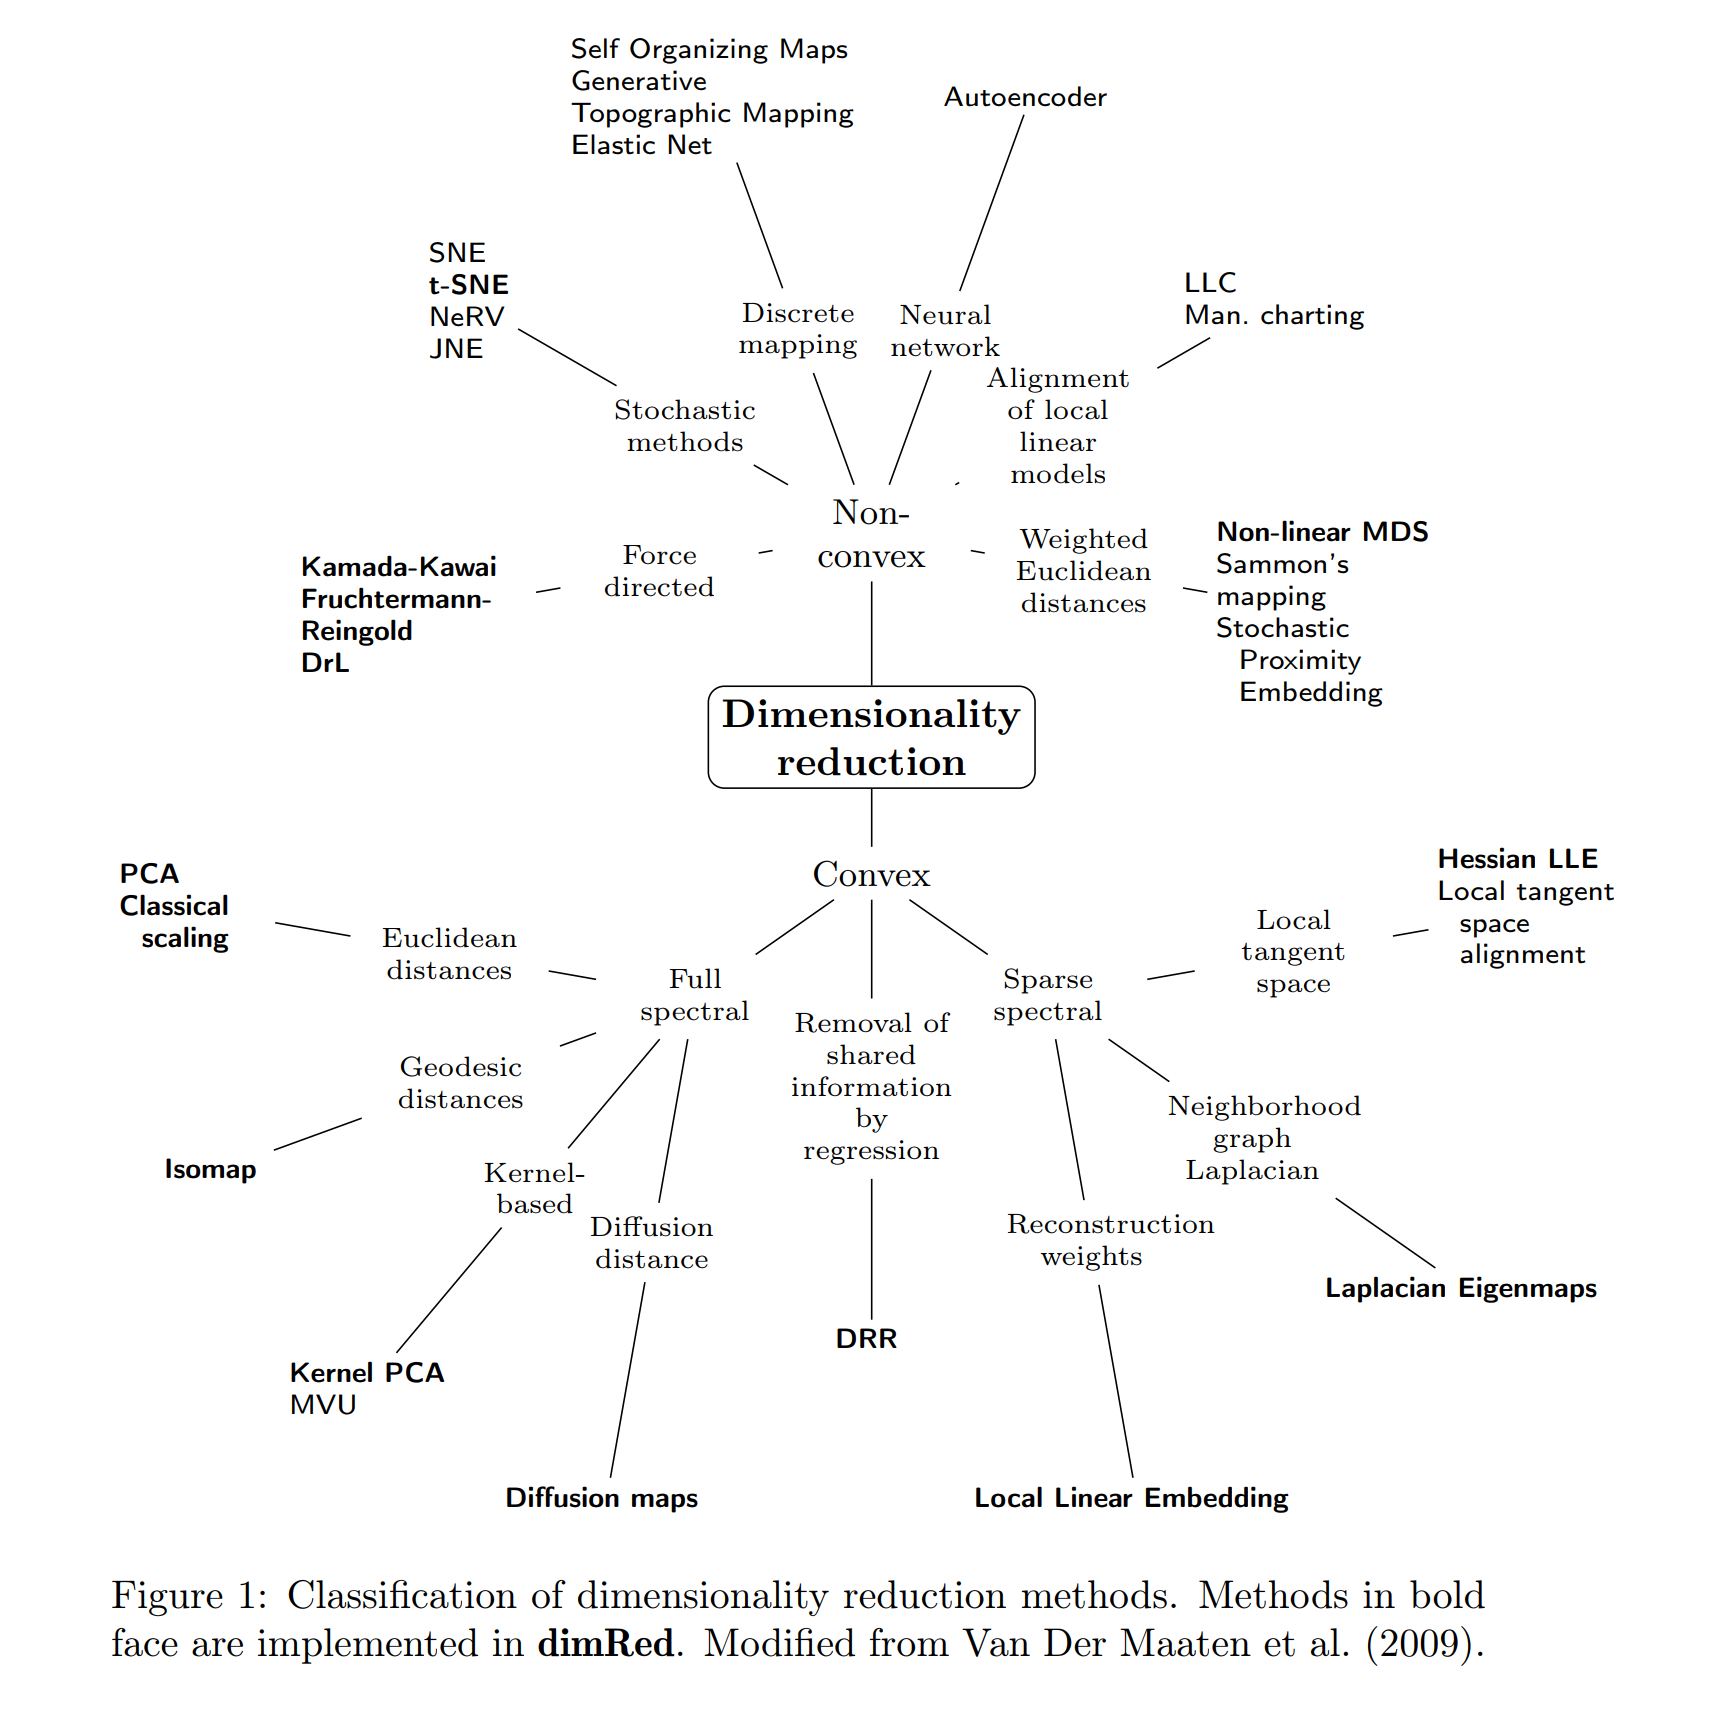
\includegraphics{pics/dim_red.png}

\end{document}
